
This \stone showcases the MINI, $P_2\times P_1$, $Q_2\times Q_1$ and Crouzeix-Raviart  (Section~\ref{sec:crouzeix-raviart})
elements which are used to solve the manufactured solution problem "Donea \& Huerta" (see Section~\ref{mms1}).

The mesh is composed of $nel_x \times nel_y$ elements which are cut in half via the same diagonal (NW-SE) into 2 triangles
for simplicity.

\begin{center}
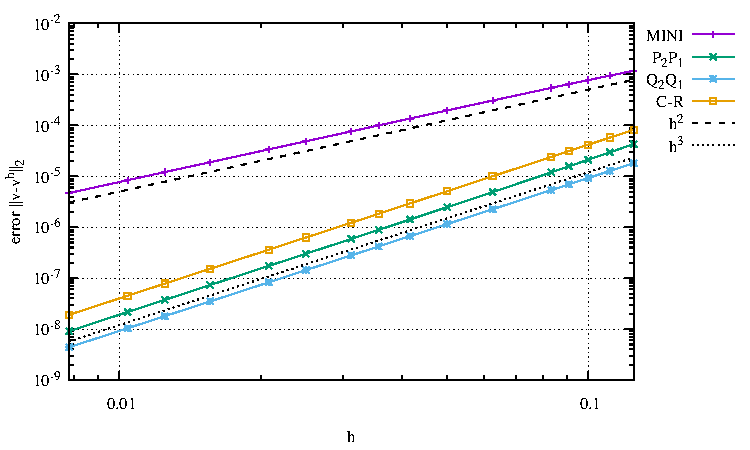
\includegraphics[width=8cm]{python_codes/fieldstone_112/results/errors_V.pdf}
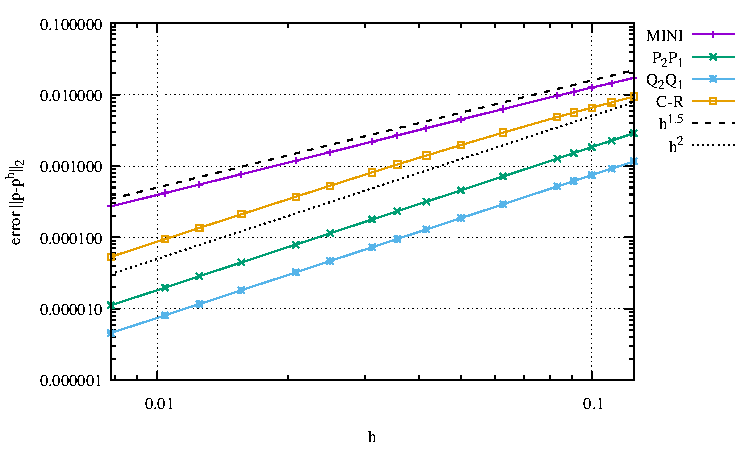
\includegraphics[width=8cm]{python_codes/fieldstone_112/results/errors_P.pdf}\\
{\captionfont Velocity (left) and pressure (right) $L_2$ error as a function of the element size $h$}
\end{center}

\begin{center}
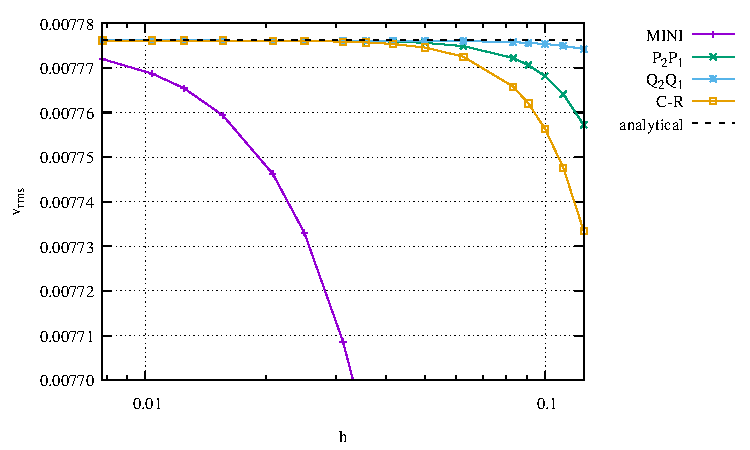
\includegraphics[width=8cm]{python_codes/fieldstone_112/results/vrms.pdf}\\
{\captionfont Root mean square velocity as a function of of the element size $h$}
\end{center}


\begin{center}
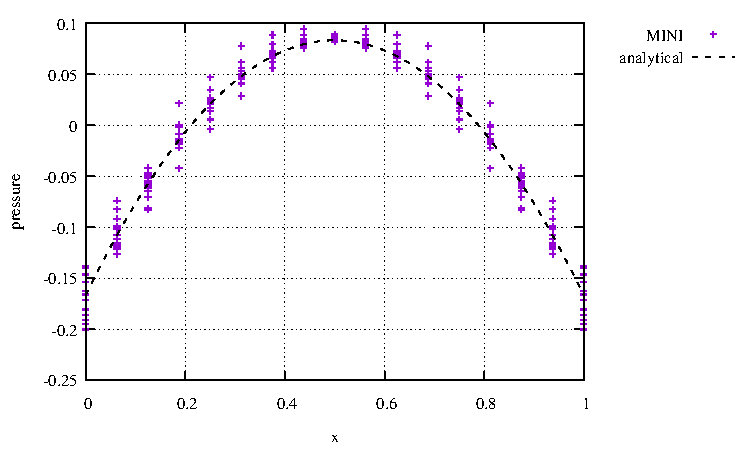
\includegraphics[width=8cm]{python_codes/fieldstone_112/results/pressMINI}
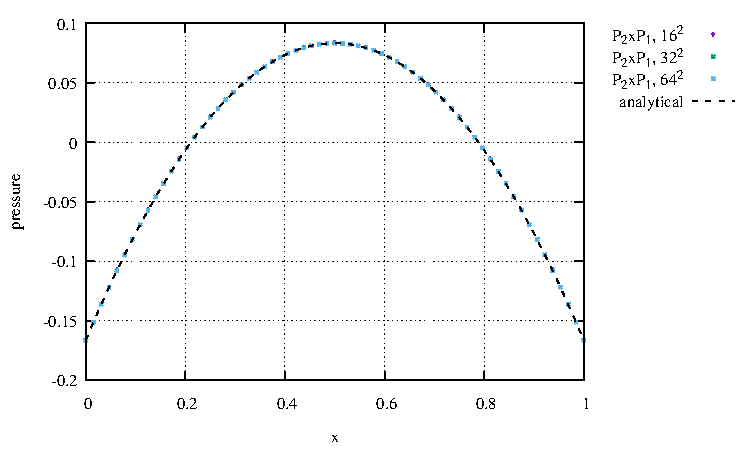
\includegraphics[width=8cm]{python_codes/fieldstone_112/results/pressP2P1}\\
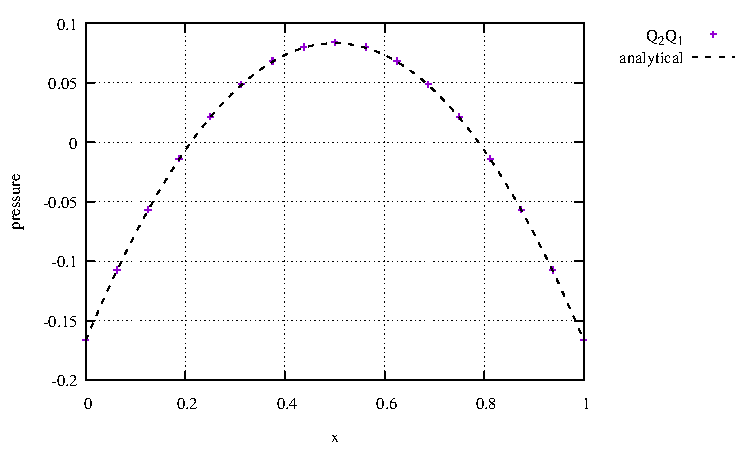
\includegraphics[width=8cm]{python_codes/fieldstone_112/results/pressQ2Q1}
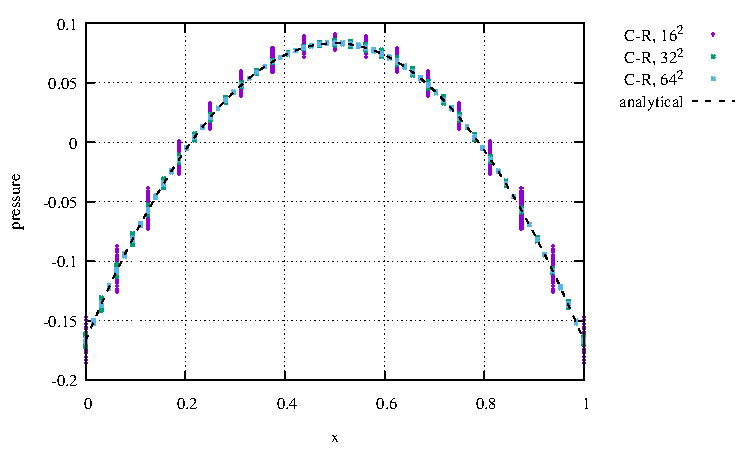
\includegraphics[width=8cm]{python_codes/fieldstone_112/results/pressCR}\\
{\captionfont Pressure field as a function of the $x$-coordinate on a 32x32 mesh.} 
\end{center}

